\documentclass{article}
\usepackage[utf8]{inputenc}
\usepackage{titling}
\usepackage{graphicx}
\usepackage{xcolor}
\usepackage[colorlinks=true,linkcolor=darkgray, urlcolor =gray]{hyperref}
\usepackage[spanish]{babel}
\DeclareUnicodeCharacter{301}{~}
\usepackage{url}


\title{Práctica 7. Aprendizaje con GeNIe.}
\author{Cristina Díaz García}
\date{Mayo 2019}

\renewcommand\maketitlehooka{\null\mbox{}\vfill}
\renewcommand\maketitlehookd{\vfill\null}


\begin{document}

\addcontentsline{toc}{section}{Índice general}

\begin{titlingpage}
\maketitle
\end{titlingpage}

\newpage

\tableofcontents

\newpage

\section{Enunciado}

\textbf{\underline{Tarea:}} Contesta a las preguntas que figuran a continuación

\textbf{\underline{Entrega:}} Documento pdf con la solución (capturas de pantalla y textos descriptivos)

\section{Pregunta 1}

Indica el valor de log(p) que te ha dado en el proceso de aprendizaje.

\subsection{Solución proporcionada}

\begin{center}
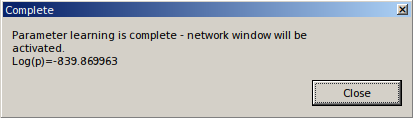
\includegraphics[scale=0.5]{images/log.png}
\end{center}

\section{Pregunta 2}

Supón un nuevo ejemplo en el que Tstsc toma el valor de más de 78; Top 10 más de 75); Pacc más de 54, Spend más de 33376, Strat menos de 19; Salar más de 74900 y Rejr más de 66. Calcula la probabilidad del nodo Apret para este ejemplo (captura la pantalla que muestra las probabilidades), y di cómo se clasificaría este ejemplo.

\subsection{Solución proporcionada}

Las probabilidades están repartidas uniformemente, y no se podría clasificar por eso mismo: las probabilidades son exactamente iguales.

\begin{center}
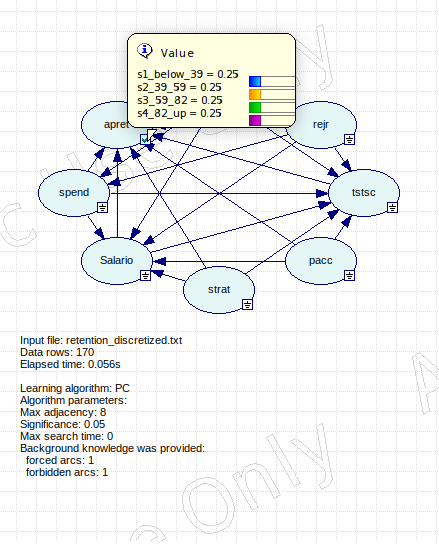
\includegraphics[scale=0.4]{images/learning.png}
\end{center}

\section{Pregunta 3}

Repite lo pedido en la pregunta 2, con el modelo Naive Bayes obtenido.

\subsection{Solución proporcionada}

Se clasificaría como mayor de 82, ya que tiene el 100\% de probabilidad.

\begin{center}
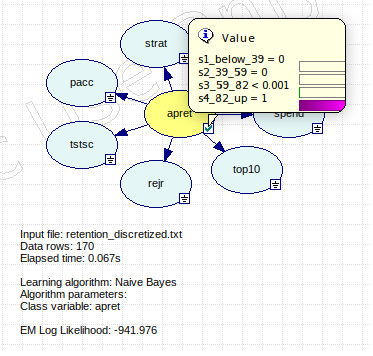
\includegraphics[scale=0.5]{images/ej3.png}
\end{center}

\section{Pregunta 4}

Escribe un breve informe acerca de la calidad del modelo aprendido, tanto para el caso de redes bayesianas como el modelo Naive Bayes (incluye también los valores obtenidos para el área bajo la curva ROC, en ambos casos). A la vista de los resultados obtenidos, ¿qué modelo es mejor?

\subsection{Solución proporcionada}

Ambos modelos tiene una calidad bastante buena, por lo que si tuvieramos que elegir uno, lo elegiríamos por su simplicidad: Naive Bayes.

\newpage
\textbf{Redes Bayesianas}

\begin{center}
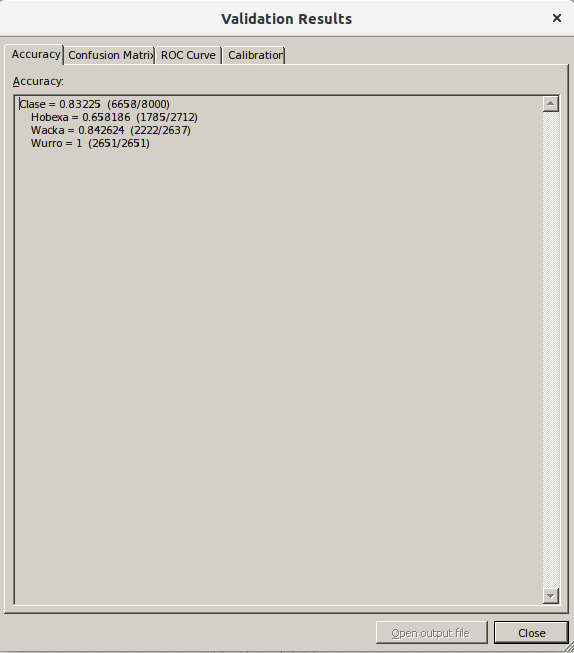
\includegraphics[scale=0.4]{images/4a.png}
\end{center}

\begin{center}
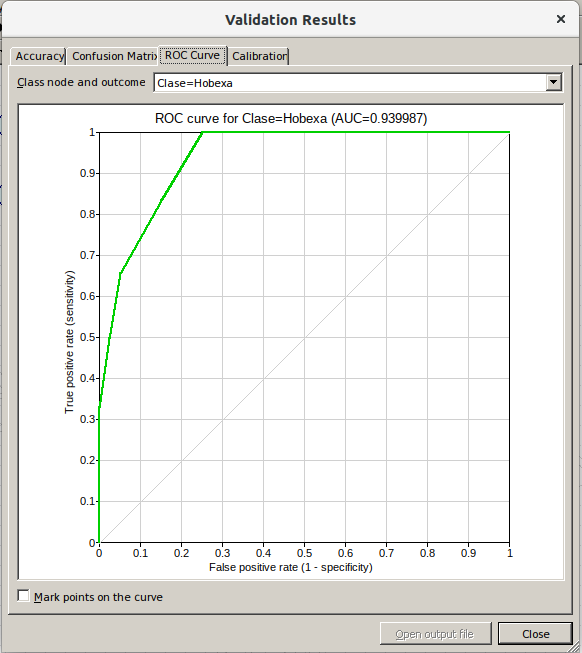
\includegraphics[scale=0.4]{images/4c.png}
\end{center}

\begin{center}
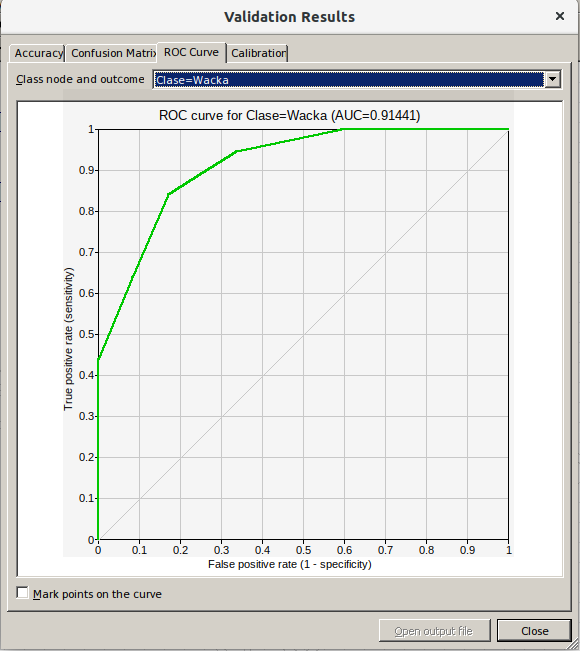
\includegraphics[scale=0.4]{images/4w1.png}
\end{center}

\begin{center}
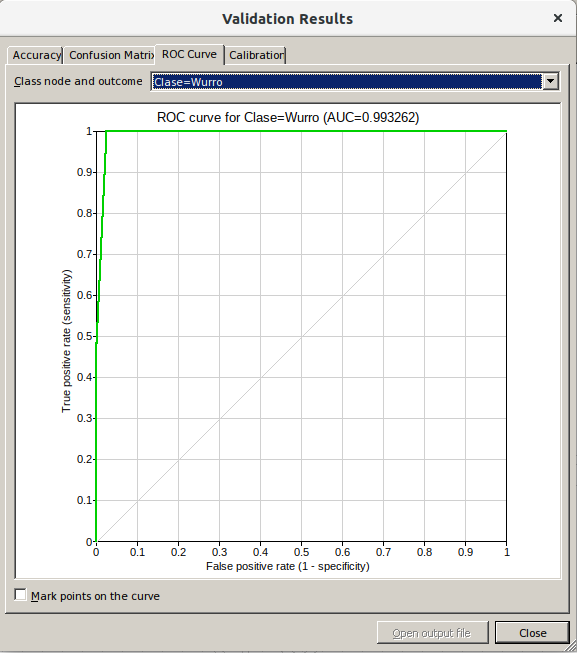
\includegraphics[scale=0.4]{images/4w2.png}
\end{center}

\newpage
\textbf{Naive Bayes}

\begin{center}
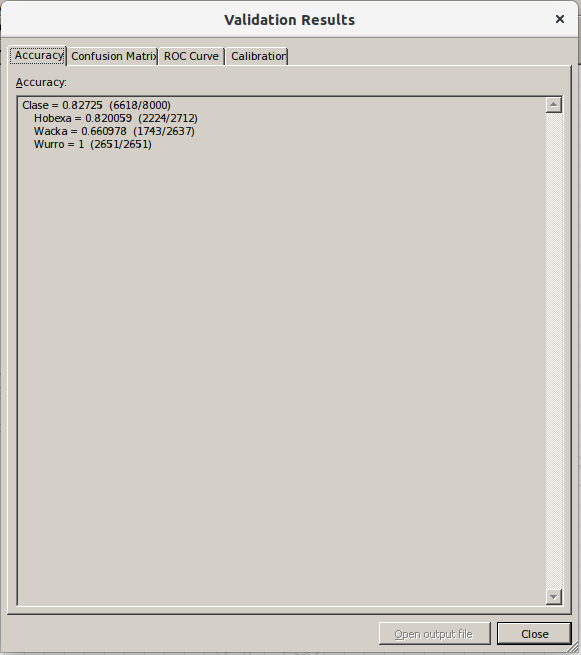
\includegraphics[scale=0.4]{images/4e.png}
\end{center}

\begin{center}
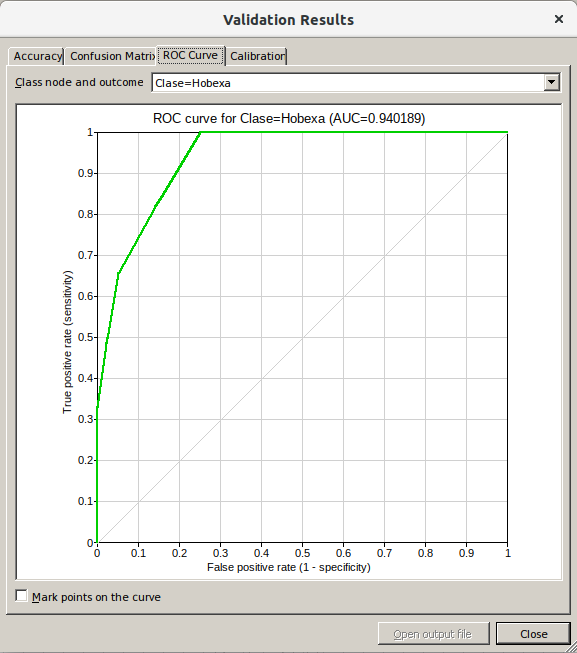
\includegraphics[scale=0.4]{images/4g.png}
\end{center}

\begin{center}
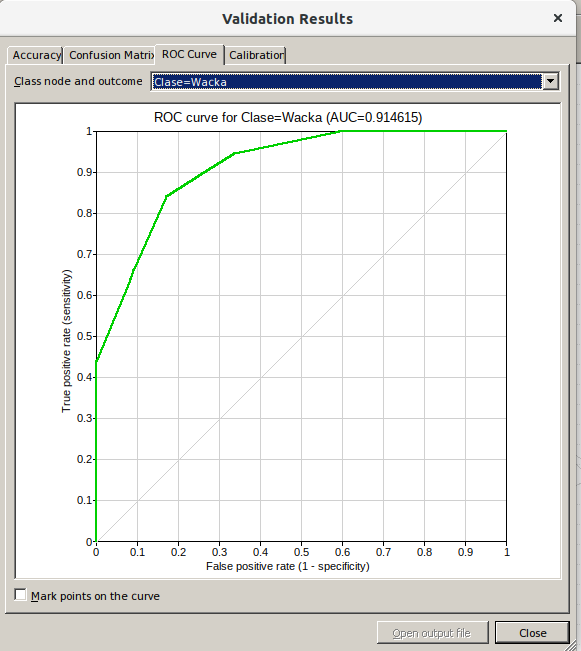
\includegraphics[scale=0.4]{images/4w3.png}
\end{center}

\begin{center}
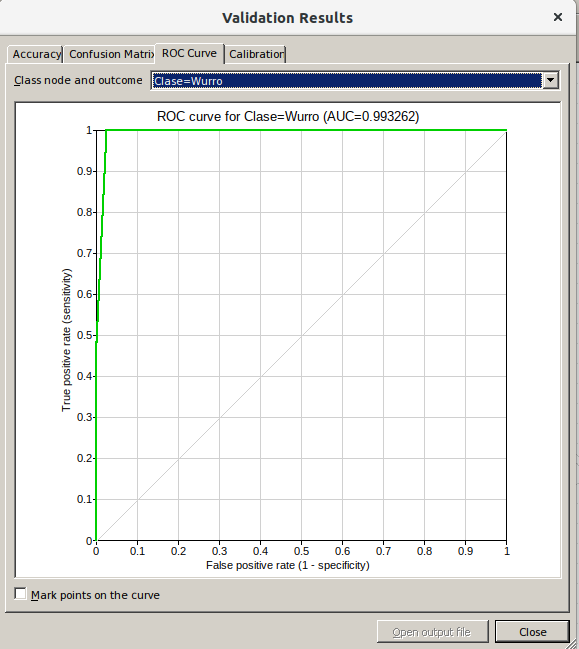
\includegraphics[scale=0.4]{images/4w4.png}
\end{center}

\begin{thebibliography}{9}
\bibitem{Bayes} Información oficial de GeNIe, \url{https://www.bayesfusion.com}.
\end{thebibliography}

\end{document}